\documentclass{article}
\usepackage[headheight=40pt, textheight=560pt]{geometry}
\usepackage{paralist}
\usepackage{scalerel,amssymb}
\usepackage{amsmath}
\usepackage{colortbl}
\usepackage{array}
\usepackage{multirow}
\usepackage{blindtext}
\usepackage{reledmac}
\usepackage{changepage}

\usepackage{pgfplots}
\usepackage{tikz}
\usetikzlibrary{positioning}
\usetikzlibrary{shapes.geometric, arrows}
\tikzstyle{arrow} = [thick,->,>=stealth]

\usepackage{graphicx}
\usepackage{stix}

\newcommand{\tableflip}{$($\rotatebox{45}{$\smile$}$^{\circ}\smwhtsquare^{\circ})\rotatebox{45}{$\smile$}\mkern-6mu\frown$\raisebox{0.5ex}{$\bot$}$\mkern-3.5mu-\mkern-3.5mu$\raisebox{0.5ex}{$\bot$}}

\usepackage{stackengine}
\def\apeqA{\SavedStyle\sim}
\def\apeq{\setstackgap{L}{\dimexpr.5pt+1.5\LMpt}\ensurestackMath{%
  \ThisStyle{\mathrel{\Centerstack{{\apeqA} {\apeqA} {\apeqA}}}}}}

\usepackage{fancyhdr}
\fancyhead[L]{
	\begin{tabular}{lll}
		\begin{tabular}{l}
			\includegraphics[scale=0.07]{security_lock}
		\end{tabular}	
		&
		\begin{tabular}{l}
			\LARGE \textbf{Cryptography} \\
			\Large \textsc{Zusammenfassung}
		\end{tabular}
		&
		\begin{tabular}{l}
			\tableflip
		\end{tabular}
	\end{tabular}
}
\fancyhead[R]{16-124-836 \\
Marcel \textsc{Zauder}}
\renewcommand{\headrulewidth}{0.4pt}
\fancyfoot[C]{\thepage}
\renewcommand{\footrulewidth}{0.4pt}

\usepackage{hyperref}

\begin{document}
	\pagestyle{fancy}
	\section{One Time Pad}
		\begin{adjustwidth*}{2em}{}
			\subsection{What is [\textsc{not}] \textsc{Cryptography}}
			\begin{adjustwidth*}{2em}{}
				\subsubsection{Introduction}
					\begin{adjustwidth*}{2em}{4em}
						In the idealized model we assume that Alice wants to send a message $m$ (\textit{privately}) to Bob. Alice will modify the message $m$, also called \textit{\textbf{plaintext}}, with any method to create a \textit{\textbf{ciphertext}} $c$ which will be actually sent to Bob. This transformation is also called encryption (\textit{\textbf{Enc}}). After receiving the ciphertext $c$, Bob will reverse the step of transforming by using a decription algorithm (\textit{\textbf{Dec}}) to (\textit{hopefully}) get the original plaintext $m$. \\
						\textit{\textbf{\textsc{Note:}}} We are not trying to hide that a message is sent, so an \textbf{\textsc{Eavesdropper}} (an attacker between Alice and Bob) can obtain the ciphertext $c$ at any instance. Hiding the existence of communication is called \textit{steganography}.
						\\
						\begin{adjustwidth*}{1em}{}
							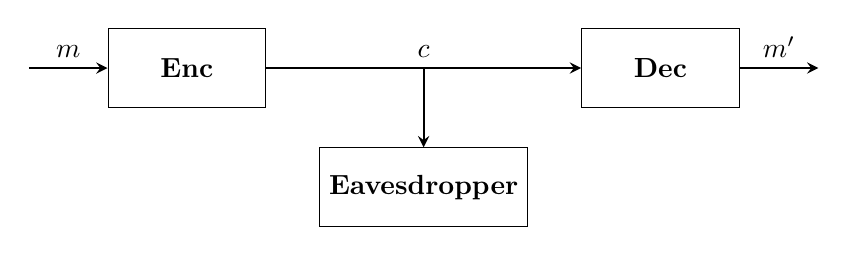
\begin{tikzpicture}
								\coordinate (start);
							
								%Nodes
								\node (rect) [draw,thin,minimum width=2cm,minimum height=1cm, right=of start] (Enc) {\textsc{\textbf{Enc}}};
								\node (rect) [draw,thin,minimum width=2cm,minimum height=1cm, right=4cm of Enc] (Dec) {\textsc{\textbf{Dec}}};
								\node (rect) [draw,thin,minimum width=2cm,minimum height=1cm, below right=0.5cm and 0.675cm of Enc] (Eve) {\textsc{\textbf{Eavesdropper}}};
								\node [right=of Dec] (stop) {};
							
								%Lines
								\draw[arrow] (start) -- node[ anchor=south ]{$m$} (Enc.west);
								\draw[arrow] (Enc.east) -- node[ anchor=south ]{$c$} (Dec.west);
								\draw[arrow] (Enc.east) -| (Eve.north);
								\draw[arrow] (Dec.east) -- node[ anchor=south ]{$m'$} (stop.west);
							
							\end{tikzpicture}
						\end{adjustwidth*}
					\end{adjustwidth*}
				\subsubsection{Kerckhoff's principle}
				\begin{adjustwidth*}{2em}{4em}
					\textit{The method must not be required to be secret, and it must be able to fall into the enemy's hands without causing any inconvenience.} \\ \\
					So if the algorithm do not need to be secret, there must be additional information in the system, which is kept secret from any \textsc{\textbf{Eavesdropper}}. This information is called a \textbf{(secret) key} $k$. 
					\\
					\begin{adjustwidth*}{1em}{}
						\begin{tikzpicture}							
							%Nodes
							\node (rect) [draw,thin,minimum width=2cm,minimum height=1cm, right=of start] (KeyGen) {\textsc{\textbf{KeyGen()}}};
							\node [below=of KeyGen] (start) {};
							\node (rect) [draw,thin,minimum width=2cm,minimum height=1cm, right=of start] (Enc) {\textsc{\textbf{Enc}}};
							\node (rect) [draw,thin,minimum width=2cm,minimum height=1cm, below right=0.5cm and 0.675cm of Enc] (Eve) {\textsc{\textbf{Eavesdropper}}};
							\node (rect) [draw,thin,minimum width=2cm,minimum height=1cm, right=4cm of Enc] (Dec) {\textsc{\textbf{Dec}}};
							\node [right=of Dec] (stop) {};
							
							%Lines
							\draw[arrow] (KeyGen.east) -| node[ anchor=south ]{$k$} (Enc.north);
							\draw[arrow] (KeyGen.east) -| node[ anchor=south ]{$k$} (Dec.north);
							\draw[arrow] (start) -- node[ anchor=south ]{$m$} (Enc.west);
							\draw[arrow] (Enc.east) -- node[ anchor=south ]{$c$} (Dec.west);
							\draw[arrow] (Enc.east) -| (Eve.north);
							\draw[arrow] (Dec.east) -- node[ anchor=south ]{$m'$} (stop.west);
							
						\end{tikzpicture}
					\end{adjustwidth*}
				\end{adjustwidth*}
			\end{adjustwidth*}
		\end{adjustwidth*}
		\hfill \\ \\ \\
		\begin{adjustwidth*}{2em}{}
			\subsection{Specifics of \textsc{One-Time Pad}}
			\begin{adjustwidth*}{2em}{4em}
				A \textit{one-time pad} often uses a secret key in the form of a bit string of length $\lambda$. The plain- and ciphertexts are also $\lambda$bit-strings. \\
				The construction of such an one-time pad looks as follows:
				\\
				\begin{adjustwidth*}{2em}{}
					\begin{tabular}{lllll}
						\begin{tabular}{|l|}
							\hline
							\underline{\textsc{KeyGen()}} \\
							\ $k \leftarrow \{ 0,1 \} ^{\lambda}$ \\
							\ \textbf{return} $k$ \\
							\hline
						\end{tabular}
						&
						&
						\begin{tabular}{|l|}
							\hline
							\underline{\textsc{Enc}($k$, $m \in \{ 0,1 \} ^{\lambda}$)} \\
							\ $c := k \oplus m$ \\
							\ \textbf{return} $c$ \\
							\hline
						\end{tabular}
						&
						&
						\begin{tabular}{|l|}
							\hline
							\underline{\textsc{Dec}($k$, $c \in \{ 0,1 \} ^{\lambda}$)} \\
							\ $m' := k \oplus c$ \\
							\ \textbf{return} $m'$ \\
							\hline
						\end{tabular}
					\end{tabular}
				\end{adjustwidth*}
				\hfill \\
				Recapture that $k \leftarrow \{ 0,1 \} ^{\lambda}$ means that $k$ is sampled uniformly from the set of $\lambda$bit-strings. \\
				Further we claim that for all $k,m \in \{ 0,1 \} ^{\lambda}$ it is true, that $Dec(k,Enc(k,m)) = m$. \\
				Otherwise the usage of one-time pad would be silly. \\
				For security reasons we want to say about the encryption scheme that an \textsc{Eavesdropper} (who does not know $k$) cannot leran anything about the message $m$. \\
				In the end we need to claim that an encryption algorithm is secure if for every $m \in \{ 0,1 \} ^{\lambda}$ the distribution \textsc{Eavesdrop}($m$) is the \textbf{uniform distribution} of $\{ 0,1 \} ^{\lambda}$, explicitly for every $m,m' \in \{ 0,1 \} ^{\lambda}$ the distributions \textsc{Eavesdrop}($m$) and \textsc{Eavesdrop}($m'$) are identical.
			\end{adjustwidth*}
		\end{adjustwidth*}
		
	\section{The Basics of Proveable Security}
		\begin{adjustwidth*}{2em}{}
		\end{adjustwidth*}
	
\end{document}